% #################
% ### PREAMBLE  ###
% #################

\RequirePackage[l2tabu,orthodox]{nag}

\documentclass[headsepline,footsepline,footinclude=false,oneside,fontsize=11pt,paper=a4,listof=totoc,bibliography=totoc]{scrbook} % one-sided

\PassOptionsToPackage{table,svgnames,dvipsnames}{xcolor}

\usepackage[utf8]{inputenc}
\usepackage[T1]{fontenc}
\usepackage[sc]{mathpazo}
\usepackage[american]{babel}
\usepackage[autostyle]{csquotes}
\usepackage[%
  backend=biber,
  bibwarn,
  url=false,
  style=numeric,
  maxnames=4,
  maxbibnames=99,
  maxcitenames=1,
  firstinits,
  uniquename=init,
  abbreviate=false,
  doi=false,
  isbn=false]{biblatex}
\usepackage{listings}
\usepackage{lstautogobble}
\usepackage{booktabs}
\usepackage[final]{microtype}
\usepackage[toc,nonumberlist,acronym]{glossaries}
\renewcommand*{\glspostdescription}{} %Den Punkt am Ende jeder Beschreibung deaktivieren

\usepackage{amsmath,amssymb,marvosym} % Math

\usepackage{lipsum} % Lorem ipsum. You can safely remove this when you entered your content!

%\usepackage{fancyhdr}

%\usepackage{xspace} % Für manuelle Abstände

% PDF
\usepackage[pdfauthor={YOUR NAME},
	pdftitle={YOUR TITLE},
	baseurl={http://campar.in.tum.de},
	breaklinks,hidelinks]{hyperref}

\usepackage{url}
%\usepackage{pdflscape} % einzelne Seiten drehen können

% Tabellen
%\usepackage{multirow} % Tabellen-Zellen über mehrere Zeilen
%\usepackage{multicol} % mehre Spalten auf eine Seite
%\usepackage{tabularx} % Für Tabellen mit vorgegeben Größen
%\usepackage{longtable} % Tabellen über mehrere Seiten
%\usepackage{array}
%\usepackage{float}
%\usepackage{rotating} % Tabellen im Querformat

% Bilder
\usepackage{graphicx} % Bilder
\usepackage{color} % Farben
%\usepackage{floatflt} % Textumfluss
\usepackage{caption} % Verbesserte Untertitel
\usepackage{subfigure} % mehrere Abbildungen nebeneinander/übereinander
%\newcommand{\subfigureautorefname}{\figurename} % um \autoref auch für subfigures benutzen
\usepackage[all]{hypcap} % Beim Klicken auf Links zum Bild und nicht zu Caption gehen
%\usepackage[section]{placeins} % Bilder nur in zugehöriger Section unterbringen

\usepackage{scrhack} % necessary for listings package

\usepackage[nohints]{minitoc} % Table of content at each chapter
\usepackage{ifthen}
\usepackage{enumitem}
\setkomafont{disposition}{\normalfont\bfseries} % use serif font for headings
\linespread{1.05} % adjust line spread for mathpazo font

% Settings for glossaries
\renewcommand*{\partpagestyle}{empty}
\renewcommand{\glsnamefont}[1]{\normalfont\bfseries #1} % use serif font for glossary entry titles
\makeglossaries{}

% Mini tables of content at a chapter
\dominitoc
% Only subsections in main TOC (no subsub)
\setcounter{tocdepth}{2}

\graphicspath{{figures/}}
\DeclareGraphicsExtensions{.pdf,.png,.jpg} % bevorzuge pdf-Dateien

% PDF-Kompression
\pdfminorversion=6
%\pdfobjcompresslevel=1

% Settings for pgfplots
%\pgfplotsset{compat=1.9} % TODO: adjust to your installed version
%\pgfplotsset{
%  % For available color names, see http://www.latextemplates.com/svgnames-colors
%  cycle list={CornflowerBlue\\Dandelion\\ForestGreen\\BrickRed\\},
%}

% Settings for lstlistings
% Quellcode
\definecolor{grau}{gray}{0.25}
\definecolor{codegreen}{RGB}{28,172,0} 
\definecolor{codepink}{RGB}{170,55,241}
\lstset{
	extendedchars=true,
	basicstyle=\tiny\ttfamily,
	keywordstyle=\color{blue},
	morekeywords={properties,SetAccess,classdef,private,methods,Static,Hidden,Access,assert,parfor},
	tabsize=2,
	stringstyle=\color{codepink},
	showstringspaces=false,%without this there will be a symbol in the places where there is a space
	commentstyle=\color{codegreen},
	numbers=left,
	numberstyle={\tiny \color{black}},% size of the numbers
	numbersep=9pt, % this defines how far the numbers are from the text	
	% für schönen Zeilenumbruch
	breakautoindent  = true,
	breakindent      = 2em,
	breaklines       = true,
	postbreak        = ,
	prebreak         = \raisebox{-.8ex}[0ex][0ex]{\Righttorque},
}

% für autoref von Gleichungen in itemize-Umgebungen
\makeatletter
\newcommand{\saved@equation}{}
\let\saved@equation\equation
\def\equation{\@hyper@itemfalse\saved@equation}
\makeatother 
% Basic information for cover & title page
\newcommand*{\getUniversity}{Technische Universität München}
\newcommand*{\getFaculty}{Department of Informatics}
\newcommand*{\getTitle}{YOUR THESIS TITLE in ENGLISH}
\newcommand*{\getTitleGer}{YOUR THESIS TITLE in GERMAN}
\newcommand*{\getAuthor}{Dhaval Shah}
\newcommand*{\getDoctype}{Master's Thesis in Biomedical Computing}
\newcommand*{\getSupervisor}{Prof.~Dr.~Bjoern~Menze}
\newcommand*{\getAdvisor}{Suprosanna Shit}
\newcommand*{\getSubmissionDate}{\today}
\newcommand*{\getSubmissionLocation}{München}
	
% #################
% ### SHORTCUTS ###
% #################

\newcommand{\TUM}{Technische Universit\"at M\"unchen}

\newcommand{\bigLineSpacing}[1]{
	\ifthenelse{\equal{#1}{ON}}{
		% Flexible whitespace between paragraphs
		\setlength{\parskip}{3mm plus4mm minus2mm}
		\linespread{1.1}
	}{
		% Whitespace OFF
		\setlength{\parskip}{0mm}
		\linespread{1.0}
	}
}

% Todos in text
\newcommand{\todo}[1]{
	{\color{red} TODO: #1} \normalfont
}
\newcommand{\info}[1]{
	{\colorbox{blue}{\color{white}(INFO: #1)}}
}
\newcommand{\delete}[1]{
	{\color{blue} DELETE?: #1} \normalfont
}

% Easy acronym
\newcommand{\acr}[2] {
	\newacronym{#1}{#1}{#2}
}

% Fixed-width image
\newcommand{\img}[4]{
	\begin{figure}[!hbt]
		\centering
		\vspace{1ex}
		\includegraphics[width=#2]{figures/#1}
		\caption[#4]{#3}
		\label{fig:#1}
		\vspace{1ex}
	\end{figure}
}
% Image with file width
\newcommand{\imgfile}[3]{
	\begin{figure}[!hbt]
		\centering
		\vspace{1ex}
		\includegraphics{figures/#1}
		\caption[#3]{#2}
		\label{fig:#1}
		\vspace{1ex}
	\end{figure}
}
% Bild todo
\newcommand{\todoimg}[2]{
	\begin{figure}[!hbt]
		\centering
		\vspace{2ex}
		\includegraphics[width=6cm]{settings/todo}
		\caption{\todo{#2}}
		\label{fig:#1}
		\vspace{2ex}
	\end{figure}
}
% Image on the right side
\newcommand{\imgright}[4]
{
	\begin{floatingfigure}[r]{#2}
		%\centering
		\includegraphics[width=#2]{figures/#1}
		\captionsetup{width=#2}
		\caption[#4]{#3}		
		\label{fig:#1}
	\end{floatingfigure}
}

%\bibliography{bibliography/literature}
\bibliography{bibliography/library}

\newglossaryentry{lwr}
{
  name={glossary},
  description={is a list of definitions for special terms in your thesis},
  name={intracranial aneurysm},
  description={bulge located in a blood vessel in the brain}
}

\acr{TUM}{Technische Universität München}
\acr{UIA}{Unruptured Intracranial Aneurysm} 
\acr{CT}{Computed Tomography}
\acr{MRA}{Magnetic Resonance Angiography}
\acr{TOF}{Time-of-Flight}
\acr{ADAM}{Aneurysm Detection And segMentation}
\acr{3D-RA}{3D X-ray Rotational Angiography}
\acr{SVM}{Support Vector Machine}

% #################
% ### SETTINGS  ###
% #################

\begin{document}
	
\input{pages/cover}

\frontmatter{}

\input{pages/title}
\input{pages/disclaimer}

\bigLineSpacing{ON}
\chapter*{\abstractname}

Accurate segmentation of unruptured intracranial aneurysms (UIAs) is important to quantify aneurysms and assess risk of rupture to allow informed treatment and planning decisions to be made \cite{White2001}. Introducing a reliable, automatic 3D segmentation method could be beneficial to improve aneurysm quantification for this purpose. The Triplanar-Net architecture was therefore designed for the task of segmenting UIAs in 3D TOF-MRA images, with the aim of also reducing inference time and required resources for producing an accurate segmentation.

The dataset made available as part of the MICCAI2020 ADAM challenge by \citeauthor{Timmins2020} was used to train Triplanar-Net for the segmentation, and the network was submitted for evaluation on the non-publicly available dataset. Two other networks that have been used previously for this task are also explored, and evaluated -- DeepMedic and nnU-Net, with nnU-Net being the winning submission to the challenge. The train dataset consisted of 113 cases with a total of 129 aneurysms, with both negative and positive cases being present (cases with and without aneurysms).

The basis of Triplanar-Net is to use 2D MIP projections in the axial, coronal and sagittal views to produce a 3D binary output segmentation of a TOF-MRA volume, with pixels labelled as foreground representing segmented aneurysms. By using 2D inputs, the trainable parameters of the network can be drastically reduced and the overall inference time also improved.

The task of segmentation was evaluated using the dice similarity coefficient (DSC), modified hausdorff distance (95th percentile) (MHD), and volumetric similarity (VS), and reported over the train and test dataset for the nnU-Net, DeepMedic and Triplanar-Net architectures.

Based on segmentation metrics, the proposed Triplanar-Net is not able to perform on par with the SOTA but is able to perform better than the DeepMedic architecture. This suggests that further work needs to be done in attempting to use 2D projections for 3D segmentations, and also that this proposed network cannot be recommended to be used in a clinical setting as it is presented.
%\bigLineSpacing{OFF}

\microtypesetup{protrusion=false}
\tableofcontents{}
\microtypesetup{protrusion=true}

%\bigLineSpacing{ON}

\mainmatter{}
	
% #################
% ### CHAPTERS  ###
% #################

\chapter{Introduction}

%\minitoc\pagebreak


\section{Background}
An intracranial aneurysm is a bulge located in a blood vessel in the brain, and the rupture of an intracranial aneurysm is a very serious incident that has high fatality and morbidity rates \todo{add ref + details}. Unruptured intracranial aneurysms (UIAs) affect approximately $3$-$5 \%$ of the adult population, irrespective of geographical location and/or ethnicity \cite{vlak2011prevalence}. The clinical manifestations of UIAs however, are subtle, with only approximately $10$-$15\%$ of intracranial aneurysms being symptomatic \cite{friedman2001small}. \todo{risk of rupture of aneurysm} Therefore, the diagnosis of an intracranial aneurysm is primarily done through the use of imaging modalities such as intra-arterial digital subtraction angiography (IADSA), computed tomography angiography (CTA) and magnetic resonance angiography (MRA). The diagnosis of aneurysm before symptoms arise allows possible intervention, if deemed necessary based on size and location \todo{ref}. \todo{risk factors?} \todo{differences in imaging modalities?}

\section{Motivation}
Due to rapidly growing workload of radiologists and radiology department, it could be beneficial to introduce a reliable method for automated detection of UIAs from diagnostic images of patients.\todo{refs} \todo{more}


\section{Goal}
Design a neural network. Also, focus on trying to reduce need for large computations by attempting to use 2d networks, but still reproduce aneurysm segmentations in 3d. \todo{elaborate and extend}








\chapter{Related Work}
\label{chapter2}
%\minitoc\pagebreak
% Aim for 6-9 pages

Several methods and algorithms have been published that tackle segmentation of UIAs, as well as detection. To easily discuss them they can be separated into non-deep learning and deep-learning based methods. Although in this work the focus is on segmentation of aneurysms, it is also important to analyze methods of detection as some of the work done in that field can also be applied to segmentation. There are also a variety of methods that are not evaluated on MRA images but rather on other modalities, and these are also included.

\section{Non-deep learning-based aneurysm detection and segmentation}
Various methods have been proposed for detection of intracranial aneurysms prior to the surge of deep learning in this field. The methods include some that involve using machine learning methods with handcrafted features, as well as some that involve the use of preprocessing and filtering to detect or segment aneurysms. \citeauthor{Lauric2010} proposed automatic detection of aneurysms in CTA and 3D X-ray rotational angiography (3D RA) that utilizes the Writhe number -- used to measure how much a curve twists and coils -- to characterize surfaces \cite{Lauric2010}. However, the detection algorithm requires a segmented volume of cerebral vasculature, and a large amount of preprocessing. \citeauthor{Yang2011} similarly proposed a method that also requires the segmentation of the cerebral vasculature in the first step \cite{Yang2011}. Following this, the corresponding 3D centerline of the segmentation is computed, and used to determine vessel parts and corresponding endpoints. This serves as an initial sample of aneurysm candidates, which is further extended using thresholding, and finally the sample is reduced using a rule base. \citeauthor{Suniaga2012} in their work aimed to combine all relevant parameters used in these previous studies within one approach \cite{Suniaga2012}. Like \citeauthor{Yang2011}, their method involves computing the 3D centerline from the extracted cerebrovascular segmentation, after which a SVM is used for classification of initial aneurysm candidates based on extracted parameters. Another method proposed by \citeauthor{Hentschke2014} is one that aims to classify multimodal angiographic images (in CTA, 3D-RA, and MRA) without the required first step of segmentation that all the other previous methods employ \cite{Hentschke2014}. Following some preprocessing, Volumes of Interest (VOI) are found using connected-component analysis (CCA), and low-level and high-level features are computed on each VOI. To reduce false-positive rate, their method proposes using two variants for classification; a linear and a non-linear classification variant. The variants comprise a rule-based system followed by a linear determinant function, and either SVM, an alternate decision tree, or a LogitBoost boosting method respectively. 

The performance of these detection methods are measured using two evaluation metrics; sensitivity and false-positive rate. Sensitivity being the measure of the proportion of positives that are correctly identified, and false-positive rate being a measure of the proportion of diagnoses incorrectly classified as positive. It is possible to compare the algorithms proposed by \citeauthor{Hentschke2014}, \citeauthor{Suniaga2012}, and \citeauthor{Yang2011} -- as they use MRA images, but results reported by \citeauthor{Lauric2010} can only be compared to those reported by \citeauthor{Hentschke2014}. Nonetheless, outright comparison between the methods is still difficult. The sensitivity of the detection methods for TOF-MRA were reported above $90\%$ for all three of these studies, however \citeauthor{Hentschke2014} achieved a better sensitivity for smaller aneurysms ($< 5$ mm) of $93\%$. They were also able to detect different kinds of aneurysms (sacular and\citeauthor{Lauric2010} reported $100\%$ sensitivity compared to $95\%$ sensitivity reported by \citeauthor{Hentschke2014}. Another issue with the proposed method by \citeauthor{Hentschke2014} is the high false-positive rate in comparison with all the other studies. However, their method does not require any manual preprocessing unlike all the other proposed methods.

Non-deep learning segmentation methods have also been proposed, and they include some that are fully automatic as well as semi-automatic methods that require some form of input from the user. A semi-automatic segmentation method was proposed by \citeauthor{Firouzian2011} which uses Geodesic Active Contours (GAC) for detection of aneurysms in CTA \cite{Firouzian2011}.Their proposed method is implemented in the level set framework, in which a surface is evolved to capture the aneurysm. The evolution is steered by image intensity statistics defined around the single user-defined seed point. \citeauthor{Bogunovic2011} introduced an automatic multimodal segmentation method for aneurysms (as well as cerebral vasculature) based on Geodesic Active Regions (GAR) \cite{Bogunovic2011}. This method is similar to that of \citeauthor{Firouzian2011} in that it also uses a deformable model within the level set framework, however the method also combines region-based descriptors with gradient ones to drive the evolution toward vascular boundaries. Being an automatic segmentation method, it also does not require the manual definition of a seed point. However, their method is focused toward cerebrovascular segmentation, with the added bonus of being able to segment aneurysms and therefore is not a dedicated solution for the problem of aneurysm segmentation \todo{Explain/read more why can't compare with this method}. In a work published by \citeauthor{Sen2013}, two other aneurysm segmentation methods were evaluated and another method -- Threshold-Based Level Set (TLS) was proposed \cite{Sen2013}. TLS combines GAC and the Chan-Vese model \cite{Chan2001} within the level set framework. Their method also integrates both region and boundary information, and makes use of a global threshold and gradient magnitude to form the function that evolves the segmentation towards the cerebral aneurysm. The Chan-Vese model is used to calculate the initial threshold value, after which it is iteratively updated throughout the segmentation process. 

The norm for evaluation of segmentation methods for recent publishings involves the use of metrics such as Dice Similarity Coefficient (DSC), Hausdorff Distance (HD), and Intersection-over-Union for example. In the studies published by \citeauthor{Firouzian2011}, \citeauthor{Bogunovic2011} and \citeauthor{Sen2013} these metrics were not reported making it difficult to compare the methods, aside from the obvious issue of comparing methods targeting different modalities. From these methods, the one proposed by \citeauthor{Sen2013} is geared towards solving the problem of aneurysm segmentation -- in CTA images and not MRA images -- and also does not require the manual setting of a seed point or intensity threshold. It aims to combine the method described by \citeauthor{Firouzian2011} with another method, and thus could be assumed to be more appropriate for the problem. \todo{This is bullshit mostly}


\todo{Explain why these are interesting, what to take away from these methods, if ML methods are better than more basic ones and why/why not, and more on results.} 

\section{Deep learning-based aneurysm detection and segmentation}
Non-deep learning methods require handcrafted engineered features that are defined in terms of mathematical equations. These features are then used as inputs to models that are trained to classify, detect or segment. In comparison, deep learning algorithms can automatically learn feature representations from data, and has thus seen increasing usage in radiology \cite{Hosny2018}. Specifically in the field of intracranial aneurysm management, deep learning methods have also shown to rapidly be becoming a promising aid; not only in detection of UIAs, but also in evaluating rupture risks, and predicting treatment outcomes \cite{Shi2020}.

\citeauthor{Ueda2019} propose to use a standard ResNet-18 architecture to detect intracranial aneurysms from TOF-MRA images \cite{He2016, Ueda2019}. Firstly, training candidates are extracted by detecting arterial abnormalities from cerebral arterial curvatures. Then patches are extracted from the training data set and the network is trained with the aneurysm annotations. The study involved the use of a large amount of data acquired from four medical institutions, however all TOF-MRA images were positive (i.e. all images contained one or more aneurysm(s)). Furthermore, the method proposed uses 2D axial images rather than full 3D volumes. An algorithm proposed by \citeauthor{Joo2020} extends the one introduced by \citeauthor{Ueda2019} by detecting intracranial aneurysms in 3D TOF-MRA images using a 3D ResNet architecture \cite{He2016, Joo2020}. \todo{Pros + cons of \cite{Joo2020}}. An interesting, novel method of detection was proposed by \citeauthor{Nakao2018} for 3D MRA; a voxel-based Convolutional Neural Network (CNN) classifier is used, the inputs to which are 2D images generated from VOIs of MRA images by applying an MIP algorithm \cite{Nakao2018}. \todo{More details, pros + cons}. \todo{Talk about recent ADAM challenge}

Again, directly comparing results between studies is difficult because of the different datasets and evaluation criteria. \citeauthor{Nakao2018} achieved $94.2\%$ sensitivity with $2.6$ FPs/case, however no external test set was included and the specificity (proportion of negatives correctly identified) was not reported. The dataset used in the study for evaluation also only included positive cases. Comparatively, \citeauthor{Joo2020} achieved high sensitivity and specificity, and compared to other studies theirs was one of the few reporting a higher specificity compared to human performance ($98\%$ to $89\%$). The datasets used for evaluation also included examinations without aneurysms unlike \citeauthor{Ueda2019} and \citeauthor{Nakao2018}, and an external test set was also included in the evaluation to further demonstrate the effectiveness and robustness of their algorithm.

Studies describing methods of segmenting intracranial aneurysms using deep learning are not as abundant as for detection, despite segmentation being an important problem. \todo{Word better}. \citeauthor{Park2019} propose the HeadXNet CNN for segmentation of intracranial aneurysms from CTA volumes \cite{Park2019}. Their method incorporates an encoder-decoder structure, much like the 3D U-net architecture -- known for being a standard model used for segmentation for a variety of use cases \cite{3dunet}. \todo{pros + cons}. \citeauthor{Liu2021} used a modified U-net architecture with dense blocks (connects each layer to every other layer, allowing an identity transform in between individual layers) \cite{Liu2021}. This study focused on segmenting intracranial aneurysms in 3D rotational DSA, but it still goes to show the versatility and adaptability  of the 3D U-net architecture. A surface-based deep learning framework for segmenting intracranial aneurysms in TOF-MRA has also been proposed; unlike usual volume-based pipelines, this method performs segmentation on samples of a cerebrovascular surface representation \cite{Yang2020}. However, this framework first requires to semi-automatically obtain the surface models of the principal brain arteries. \citeauthor{Sichermann2019} propose a method for detection and segmentation of intracranial aneurysms from 3D TOF-MRA data based on an open-source neural network --  DeepMedic \cite{Sichermann2019}. The DeepMedic framework is a CNN for voxelwise classification of medical imaging data after training with 3D patches at multiple scales. Their architecture contains 2 pathways; the pathways are identical apart from the input of the second pathway being a subsampled version of the first. Their study uses a large dataset, however -- like other studies -- they only use volumes that contain aneurysms. \todo{Find ADAM2020}

The results of methods used for segmentation with deep learning methods are the most important for comparisons with the proposed architecture in chapter \ref{chapter5}. Comparing results of different modalities would not be as important as for the same modality; so the studies by \citeauthor{Yang2020}, \citeauthor{Sichermann2019} and \todo{ADAM2020} can be compared. Although not the same datasets are used in each case, \citeauthor{Sichermann2019} produce a maximum Dice Similarity Coefficient of $0.53 \pm 0.30$, \citeauthor{Yang2020} obtain a maximum Dice Similarity Coefficient of $0.76 \pm 0.27$ and \todo{ADAM2020} obtain a maximum score of $0.41$. \todo{Reason why scores are so different, and which are more important}


\todo{Discuss some pros and cons of introducing deep learning to this, maybe from \cite{Kallmes2021}}

\todo{Add \cite{Duan2020}}
\todo{Add table with all results}

\todo{Differences in domain}

\todo{3d NN's, subsection?}

\todo{hybrid (3d+2d) NN's, subsection?}

\todo{CAD, AI in intracranial aneurysm diagnosis from \cite{Shi2020}}

\todo{Table with all methods discussed with results}







\chapter{Methodology}
\chapter{Time-of-Flight Magnetic Resonance Angiography}
\label{chapter3}
% Aim for 5-7 pages
\todo{Check Keedy2006, it gives a good overview of MRA used for diagnosis as well as other modalities}
As discussed previously, Time-of-Flight (TOF) Magnetic Resonance Angiography (MRA) is an imaging modality used for diagnosis of UIAs. The following chapters will discuss deep learning methods to segment UIAs on these images, however it is also valuable to go deeper into the acquisition of these images, as well as discuss and analyse the specific images used.

\section{Dataset}
The dataset used was obtained from the Aneurysm Detection And segMentation (ADAM) Challenge 2020, a medical image analysis challenge organised as part of MICCAI 2020. The train dataset of TOF-MRAs consists of \textbf{113} cases which are split into 93 containing at least one untreated, unruptured aneurysm (35 baseline and 35 follow-up of the same subject, and 23 unique subjects), and 20 scans without intracranial aneurysms. \todo{Add images of each type} \todo{Table?} \todo{Train/Validation split?}

\section{Analysis of dataset}
\todo{Analyse dataset e.g. aneurysm sizes}

\section{Acquisition}



\section{Comparison to other modalities}
\todo{Look for some open source cranial CTA with labels}
\todo{Look for some cranial DSA, maybe ask Supro if you can use the old ones}



\newpage
\chapter{Prior Networks for Aneurysm Segmentation}
\label{chapter4}
\todo{Aim for 7 to 9 pages}

Three methods of segmentation of intracranial aneurysms using 3D neural networks are evaluated with the dataset obtained from the ADAM challenge. This includes the adapted DeepMedic framework proposed by \citeauthor{Sichermann2019} and initially by \citeauthor{deepmedic}, a standard 3D U-Net architecture initially proposed by \citeauthor{3dunet}, as well as the no-new-Net (nnU-Net) architecture proposed by \citeauthor{nnUnet} which was adapted for the \todo{ADAM challenge} and received first place. 

These networks are chosen firstly due to their performance; the 3D-Unet architecture can be used as a baseline after which the proposed network architecture in this work can be measured against, \citeauthor{Sichermann2019} also showed a good DSC with their adapted framework in their study thus making it an interesting addition for comparison, and finally the nnUnet can be regarded as the gold standard architecture due to its peak performance in \todo{ADAM challenge} -- for the same dataset used in this study.
%\minitoc\pagebreak

In the following sections the architectures used are described and shown along with the experiments run in the study, and how these architectures will be adapted to this case (if any adaptation is needed). \delete{Maybe don't need to say this}

\section{3D U-Net}
\todo{Go into \citeauthor{3dunet}}
The 3D-Unet architecture has an analysis and synthesis path -- also referred to as encoder and decoder paths -- with four steps, each with different resolutions. Each layer in the analysis path contains two convolutions with a kernel size of 3 followed by a rectified linear unit (ReLU), followed by a max pooling layer with a kernel size of 2 and a stride of 2. 


\section{DeepMedic}
The network proposed by \citeauthor{Sichermann2019} was initially devised by \citeauthor{Kamnitsas2017}; it is a dual pathway, 11-layers deep, 3D Convolutional Neural Network (CNN) originally meant for the task of brain lesion segmentation. Both pathways of the network are identical, however the inputs to the second pathway are downsampled versions of the images in the first pathway. The outputs of both pathways are concatenated before the fully connected layers and finally classified. The full pipeline is shown in \ref{fig:deep-medic.jpg} \todo{Add figure, draw out or copy from paper?}

\img{deep-medic.jpg}{\linewidth}{The neural network DeepMedic, with a 2-pathway architecture. Each layer shows the number of feature maps and their size as number $\times$ size. ReLU activation and batch normalization are also applied after each layer. The diagram is taken from \citeauthor{Sichermann2019}.}{DeepMedic architecture}

Initially, \citeauthor{Kamnitsas2017} proposed DeepMedic to efficiently incorporate both local and contextual information by using the parallel, multi-scale pathways. They also employ a fully-connected Conditional Random Field (CRF) model for final post-processing of the segmentation maps \cite{Krahenbuhl2012}. However, \citeauthor{Sichermann2019} chose to exclude that in favor of thresholding solely based on aneurysm size. Also, in the study, DeepMedic was trained solely on cases that contained intracranial aneurysms, and thus the network could prove to have worse performance on the current dataset. Aneurysms in their dataset also had a mean diameter of $7.10$ mm, much larger than the $4.11$ mm average in the current dataset, which could also further deteriorate performance. \todo{Go further into expected results, like false positive rate, inference time, resource usage}

\todo{Experiments here, including training + preprocessing compared to paper}.

DeepMedic was trained for this task as described in the paper by \citeauthor{Sichermann2019}; with a learning rate of $10^{-4}$, optimization with Adam and a Nesterov momentum of $0.6$, and a hybrid training scheme in which $90\%$ of input image segments correspond to background class and $10\%$ to aneurysm class. They considered and evaluated various pre-processing steps for the best output, however since the other two network models to be evaluated will use only one set of images, this will be the same data used for this model. \todo{write better, haven't talked about pre-processing of data yet}



\section{nnUnet}
\todo{nnUnet describe, go into detailed architecture, probably draw it myself, check if Junma paper for it for the specific challenge}
The "no-new-Net" was presented in \citeyear{nnUnet}, and it is a self-adapting framework on the basis of vanilla U-Nets.




\newpage
\section{Triplanar-Net}
\label{chapter5}

It is computationally demanding to work with three-dimensional volumetric data, and consequently with three-dimensional neural networks (such as the ones shown in chapter \ref{chapter4}); this applies even more so for the case of aneurysm segmentation where localization is difficult due to the size of aneurysms. This could be overcome by using low-resolution data or by using shallow networks, however this would adversely affect performance. Therefore the proposed network architecture works with 2D projections of patches of the volumetric data. Since we are working with cerebral TOF-MRAs for the task of aneurysm segmentation, the projections used are axial, coronal and sagittal Maximum Intensity Projections (MIPs). 

To obtain better 3D context, 3D reconstruction using the orthogonal views is carried out within the network and the network is trained on 3D labels. This removes the need to naively reconstruct the label after obtaining 2D labels, and also allows the network to learn 3D context while still being lightweight and non-resource intensive. 

The input arms (and concept of using 2D MIPs) is heavily inspired by the BtrflyNet architecture, but the input portion is made deeper and an added axial view is also used \cite{sekuboyina2018}. During inference, the sagittal and coronal output heatmaps of the BtrflyNet architecture are combined using the outer product to create a 3D heatmap. Triplanar-Net similarly uses the outer product to reconstruct a 3D volume, although this is done within the network architecture and 3D labels are also used for training the network unlike for the BtrflyNet architecture.


\subsection{Maximum Intensity Projection}
Maximum Intensity Projection is a method that consists of projecting the voxel with the highest intensity lying in the direction of the plane of projection. It allows representing three-dimensional objects in two dimensions. MIPs have several advantages: vascular structures are well defined and appear clearly as tubular branching structures, the susceptibility to noise is highly reduced due to projecting only the maximum value across a view, and through MIP the use of two dimensional images immensely reduces required resources and parameters. Figure \ref{fig:mip} shows axial, coronal and sagittal MIPs obtained from two positive cases in the dataset. 

\begin{figure}[h]
	\centering
	\begin{subfigure}{\linewidth}
		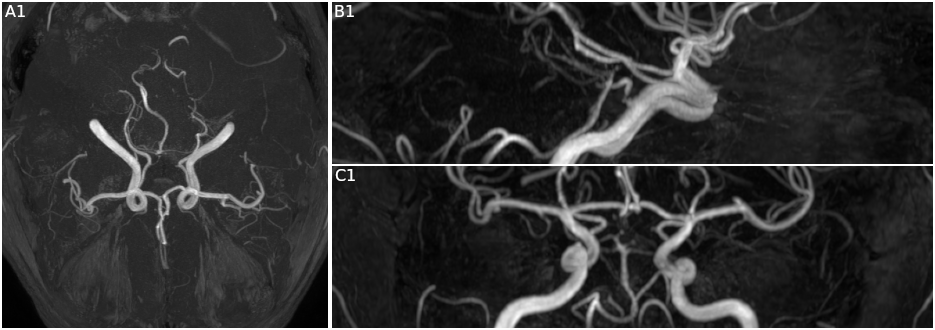
\includegraphics[width=\linewidth]{figures/mip_10021.png}
%		\phantomsubcaption
%		\label{fig:mip_10021.png}
	\end{subfigure}
	\begin{subfigure}{\linewidth}
		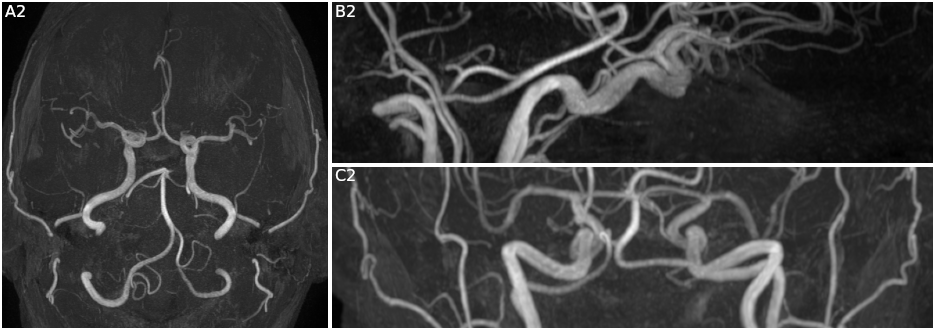
\includegraphics[width=\linewidth]{figures/mip_10028.png}
%		\phantomsubcaption
%		\label{fig:mip_10028.png}
	\end{subfigure}
	\caption[Maximum Intensity Projections of two positive cases.]{Images A1 and A2 show axial MIPs of two different cases that contain UIAs, and similarly B1, B2 and C1, C2 show sagittal and coronal views of MIPs respectively. The cases used are from the train dataset available via the ADAM challenge \cite{Timmins2020}.}
	\label{fig:mip}
\end{figure}

\begin{figure}[t]
	\centering
	\begin{subfigure}{\linewidth}
		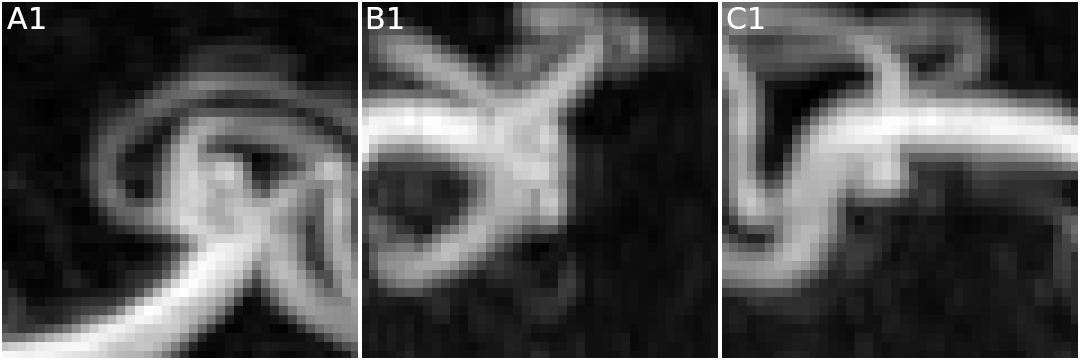
\includegraphics[width=\linewidth]{figures/mip_patch10021.png}
	\end{subfigure}
	\begin{subfigure}{\linewidth}
		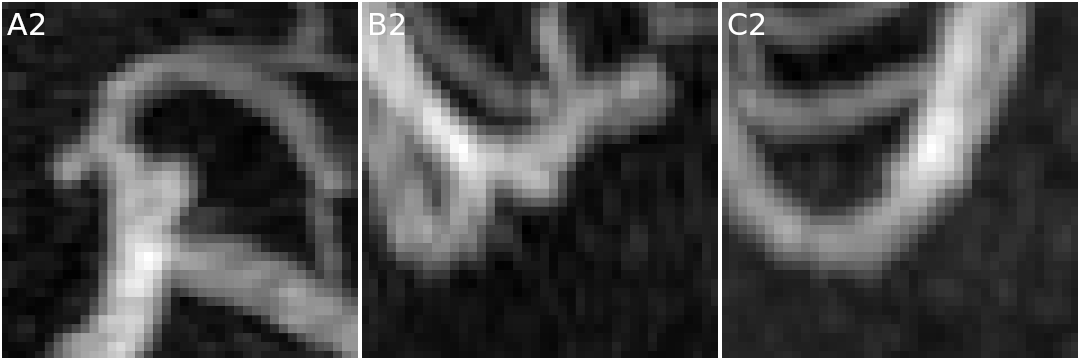
\includegraphics[width=\linewidth]{figures/mip_patch10028.png}
	\end{subfigure}
	\caption[Patches of Maximum Intensity Projections of two positive cases.]{Similarly to Figure \ref{fig:mip}, patches of axial, sagittal and coronal (A, B, and C) MIP images of two positives cases, are shown -- with the 3D patch from which the MIP is taken extracted with the aneurysm centered.}
	\label{fig:mip_patch}
\end{figure}


As discussed in chapter \ref{chapter3}, the size of aneurysms in a TOF-MRA is very small; the mean diameter of an aneurysm in our dataset being $4.11$ mm. With a re-sampled volume with voxel spacing $0.3 \times 0.3 \times 0.3$ mm\textsuperscript{3}, the mean shape of a volume encompassing an aneurysm would be $21.5 \times 21.5 \times 21.5$ -- assuming a spherical structure of the aneurysm. Axial, coronal and sagittal images (after preprocessing of the TOF-MRA volumes) would have shapes $512 \times 512$, $512 \times 140$, and $512 \times 140$ respectively. Due to this, an MIP taken of the whole three-dimensional TOF-MRA volume, would have little useful information regarding the aneurysm, such as an enlarged vessel. Therefore, as most other training procedures for other networks, Triplanar-Net is trained using patches of the whole volume. MIPs are then taken for the patch of cropped volume, further allowing the network to learn important features with respect to the aneurysm segmentation such as structure and shape. The projections the network learns from are thus as in Figure \ref{fig:mip_patch}, which are obtained from sampling a TOF-MRA volume. 

There are other projection methods, however using MIP for cerebral TOF-MRA is appropriate for this task due to the focus on vessels. \todo{is it ok to use MIP as projection method for brain volumes and why, what might be lost using 2D images, maybe contrast of TOF-MRA? etc}

\subsection{Network architecture}
The proposed Triplanar-Net is a CNN producing a binary segmentation the same size as the 3D patch used to create the MIPs. The model consists of an axial, coronal and sagittal 2D encoder path, a 2D to 3D reconstruction block, and a 3D decoder path, along with skip connections -- see the full architecture in Figure \ref{fig:trinet.pdf}. 

\img{trinet.pdf}{\linewidth}{Proposed network architecture for Triplanar-Net. Three input arms each take an MIP of either the axial, coronal or sagittal view extracted from a 3D patch. The inputs are encoded using 2D convolutions operations and max pooling before going through the 2D to 3D reconstruction block, and being decoded with 3D transpose convolutions followed by 3D convolutions. The convolution kernel size, padding size, and stride are represented as \{kernel.padding.stride\} in the image and the number of channels is shown within each block.}{Triplanar-Net architecture.}

\img{2d_to_3d.pdf}{0.5\linewidth}{Diagram of the 2D to 3D reconstruction block used in the Triplanar-Net architecture. Three inputs are given to the block -- representing the axial, sagittal and coronal MIPs. A 2D convolution with a kernel size of 3, padding 1 and stride 1 is applied to each input. The orthogonal views are then combined by taking the outer product, and a 3D convolution with kernel size of 3, padding 1 and stride 1 is applied to reconstructed 3D image.}{2D to 3D reconstruction block.}

In each encoder path a $1 \times 1$ convolution is applied to the respective input MIP, after which follow three layers containing $3 \times 3$ convolutions (with stride of 1 and padding 1) plus max-pooling with a stride of 2. 
In the the 2D to 3D reconstruction block, a convolution with kernel size $3 \times 3$ is applied to each of the feature maps of the axial, coronal and sagittal encoder paths. The 3D downsampled representation is constructed by calculating the outer product of the feature maps from the three orthogonal views, and applying a $3 \times 3 \times 3$ convolution. Figure \ref{fig:2d_to_3d.pdf} shows the 2D to 3D reconstruction block.
Lastly, to upsample the reconstructed 3D representation, the decoder path applies three layers of $4 \times 4 \times 4$ transpose convolutions (stride 2 and padding 1) followed by $3 \times 3 \times 3$ convolutions (stride 1 and padding 1). To take advantage of higher resolution features, skip connections are added that concatenate the output of each convolution operation in the encoder path to an equivalent decoder operation. As the decoder path incorporates three dimensional representations, the high-res features are also passed through their own 2D to 3D reconstruction block. The 3D binary voxelized segmentation of the aneurysm is obtained after applying a $1 \times 1 \times 1$ convolution. To introduce non-linearities to the model, each convolution operation (2D, 3D, and 3D transpose) with a kernel size greater than 1 is followed by an ELU activation function. Batch normalization is also applied after convolution operations (2D, and 3D) in the encoder and decoder paths.

Unlike the BtrflyNet architecture, Triplanar-Net constructs a 3D representation within the model (prior to the decoder path) and also does not contain a middle arm that concatenates the feature maps of the three encoder paths. Using a 3D decoder path allows the model to learn valuable 3D context when upsampling the naively reconstructed 3D feature maps, which would otherwise be lost if only 2D feature maps were involved. The parameters in the decoder path also allow to obtain a much more detailed binary segmentation, compared to that of a 2D decoder -- i.e. there would be a lot of aliasing when reconstructing a 3D output from three orthogonal MIP binary outputs for example, therefore it is more effective to create a reconstructed intermediate representation of the three projections within the network and obtain a 3D binary segmentation after decoding. 

As stated previously the axial, coronal and sagittal images used for training the network are obtained by finding the MIP in each view of a 3D patch cropped from the whole TOF-MRA volume. Multiple sampling schemes for extracting segments were tested; ultimately it was most successful to construct a training batch by extracting segments of size $32 \times 32 \times 32$ in which $90\%$ of the input samples correspond to background class and $10\%$ to foreground class (i.e. voxels containing an aneurysm). For cases in which there are no aneurysms in the TOF-MRA, all segments will only contain background class. This training strategy was employed as it reflects the most realistic distribution of foreground to background class within the data. The network is trained using dice loss which takes the form: 

\[L = 1 - \frac{2\sum_{i}^{N}p_{i}g_{i}}{\sum_{i}^{N}p_{i}^{2} + \sum_{i}^{N}g_{i}^{2}} \]

where $p_{i}$ and $g_{i}$ represent the voxel values of the predicted binary segmentation and the ground truth binary volume, summed over $N$ voxels \cite{milletari2016v}. The network is trained with 5-fold cross validation using the AdamW optimizer for 100 epochs per fold. L2 regularization of $1e-5$ is also used during training to reduce overfitting.

In comparison to the networks described in Chapter \ref{chapter4}, Triplanar-Net consists of a more shallow architecture, as well as both 2D and 3D convolutions. Generally, a shallower network can lead to poorer overall results be it for any task. However, by efficiently combining two dimensional and three dimensional data and convolutions, the network is able to be lightweight.  

Once trained, inference for a given input TOF-MRA volume proceeds as: segments of the volume are sampled on a grid, axial, coronal and sagittal MIPs are obtained for each segment and fed to the network. The output segmentation of the TOF-MRA volume is built by concatenating the network output of each segment.

%\todo{removed classifier/full pipeline part because think i can get it to work without}
%Training the network on only segments centered on the foreground (apart from negative cases) causes the network to produce segmentations with a high number of false-positives. To mitigate this as well as to allow Triplanar-Net to focus on accurate segmentation of aneurysms, it is proposed to add an initial classification step during inference on a TOF-MRA volume. The classifier evaluates whether a certain patch of the TOF-MRA volume contains a vessel with an aneurysm. If positively classified, the segment goes through to Triplanar-Net for aneurysm segmentation, and if negatively classified then no foreground pixels are segmented in the patch. The full framework for inference for any TOF-MRA volume can be seen in Figure \ref{full_pipeline.pdf}. The classifier network can also be seen in figure \todo{network for classifier}. The classifier network is trained on 3D segments of the same size as those used for training Triplanar-Net, using a uniform sampling scheme. We require that this classifier has a high sensitivity, and favors false-positives over false-negatives. Thus, it is trained using cross-entropy loss with a larger weight given to a positively classified volume. \info{elaborate/maybe write better}.
%
%\img{full_pipeline.pdf}{\linewidth}{\todo{caption}}{Full pipeline for inference.}
%
%Adding this classifier prior to Triplanar-Net is hypothesized to not heavily increase resource usage or heavily impede inference; most segments of the TOF-MRA volume will only go through one network (either the classifier or Triplanar-Net) since a very small number of segments (out of $N$ segments sampled from the TOF-MRA volume) contain an aneurysm. A segment is only processed by both the classifier and Triplanar-Net if an aneurysm is detected to be within it. The complete binary segmentation map for the TOF-MRA volume is then reconstructed by combining -- according to the coordinates of the sampled segment -- the $x$ binary segmentations from Triplanar-Net and $y$ binary segmentations that are known to not contain an aneurysm.
%
%An alternative to using this framework with a combined classifier and Triplanar-Net would be to use post-processing after obtaining the binary segmentation map of a segment and altogether not use the classifier at all. However, this was opted against as this \todo{Why not?}
%
%\todo{ablation study in appendix to show design choices, i.e. no skip blocks, no combination path, 2d decoders instead of 3d}





%\chapter{Time-of-Flight Magnetic Resonance Angiography}
\label{chapter3}
% Aim for 5-7 pages
\todo{Check Keedy2006, it gives a good overview of MRA used for diagnosis as well as other modalities}
As discussed previously, Time-of-Flight (TOF) Magnetic Resonance Angiography (MRA) is an imaging modality used for diagnosis of UIAs. The following chapters will discuss deep learning methods to segment UIAs on these images, however it is also valuable to go deeper into the acquisition of these images, as well as discuss and analyse the specific images used.

\section{Dataset}
The dataset used was obtained from the Aneurysm Detection And segMentation (ADAM) Challenge 2020, a medical image analysis challenge organised as part of MICCAI 2020. The train dataset of TOF-MRAs consists of \textbf{113} cases which are split into 93 containing at least one untreated, unruptured aneurysm (35 baseline and 35 follow-up of the same subject, and 23 unique subjects), and 20 scans without intracranial aneurysms. \todo{Add images of each type} \todo{Table?} \todo{Train/Validation split?}

\section{Analysis of dataset}
\todo{Analyse dataset e.g. aneurysm sizes}

\section{Acquisition}



\section{Comparison to other modalities}
\todo{Look for some open source cranial CTA with labels}
\todo{Look for some cranial DSA, maybe ask Supro if you can use the old ones}


%\chapter{Prior Networks for Aneurysm Segmentation}
\label{chapter4}
\todo{Aim for 7 to 9 pages}

Three methods of segmentation of intracranial aneurysms using 3D neural networks are evaluated with the dataset obtained from the ADAM challenge. This includes the adapted DeepMedic framework proposed by \citeauthor{Sichermann2019} and initially by \citeauthor{deepmedic}, a standard 3D U-Net architecture initially proposed by \citeauthor{3dunet}, as well as the no-new-Net (nnU-Net) architecture proposed by \citeauthor{nnUnet} which was adapted for the \todo{ADAM challenge} and received first place. 

These networks are chosen firstly due to their performance; the 3D-Unet architecture can be used as a baseline after which the proposed network architecture in this work can be measured against, \citeauthor{Sichermann2019} also showed a good DSC with their adapted framework in their study thus making it an interesting addition for comparison, and finally the nnUnet can be regarded as the gold standard architecture due to its peak performance in \todo{ADAM challenge} -- for the same dataset used in this study.
%\minitoc\pagebreak

In the following sections the architectures used are described and shown along with the experiments run in the study, and how these architectures will be adapted to this case (if any adaptation is needed). \delete{Maybe don't need to say this}

\section{3D U-Net}
\todo{Go into \citeauthor{3dunet}}
The 3D-Unet architecture has an analysis and synthesis path -- also referred to as encoder and decoder paths -- with four steps, each with different resolutions. Each layer in the analysis path contains two convolutions with a kernel size of 3 followed by a rectified linear unit (ReLU), followed by a max pooling layer with a kernel size of 2 and a stride of 2. 


\section{DeepMedic}
The network proposed by \citeauthor{Sichermann2019} was initially devised by \citeauthor{Kamnitsas2017}; it is a dual pathway, 11-layers deep, 3D Convolutional Neural Network (CNN) originally meant for the task of brain lesion segmentation. Both pathways of the network are identical, however the inputs to the second pathway are downsampled versions of the images in the first pathway. The outputs of both pathways are concatenated before the fully connected layers and finally classified. The full pipeline is shown in \ref{fig:deep-medic.jpg} \todo{Add figure, draw out or copy from paper?}

\img{deep-medic.jpg}{\linewidth}{The neural network DeepMedic, with a 2-pathway architecture. Each layer shows the number of feature maps and their size as number $\times$ size. ReLU activation and batch normalization are also applied after each layer. The diagram is taken from \citeauthor{Sichermann2019}.}{DeepMedic architecture}

Initially, \citeauthor{Kamnitsas2017} proposed DeepMedic to efficiently incorporate both local and contextual information by using the parallel, multi-scale pathways. They also employ a fully-connected Conditional Random Field (CRF) model for final post-processing of the segmentation maps \cite{Krahenbuhl2012}. However, \citeauthor{Sichermann2019} chose to exclude that in favor of thresholding solely based on aneurysm size. Also, in the study, DeepMedic was trained solely on cases that contained intracranial aneurysms, and thus the network could prove to have worse performance on the current dataset. Aneurysms in their dataset also had a mean diameter of $7.10$ mm, much larger than the $4.11$ mm average in the current dataset, which could also further deteriorate performance. \todo{Go further into expected results, like false positive rate, inference time, resource usage}

\todo{Experiments here, including training + preprocessing compared to paper}.

DeepMedic was trained for this task as described in the paper by \citeauthor{Sichermann2019}; with a learning rate of $10^{-4}$, optimization with Adam and a Nesterov momentum of $0.6$, and a hybrid training scheme in which $90\%$ of input image segments correspond to background class and $10\%$ to aneurysm class. They considered and evaluated various pre-processing steps for the best output, however since the other two network models to be evaluated will use only one set of images, this will be the same data used for this model. \todo{write better, haven't talked about pre-processing of data yet}



\section{nnUnet}
\todo{nnUnet describe, go into detailed architecture, probably draw it myself, check if Junma paper for it for the specific challenge}
The "no-new-Net" was presented in \citeyear{nnUnet}, and it is a self-adapting framework on the basis of vanilla U-Nets.



%\section{Triplanar-Net}
\label{chapter5}

It is computationally demanding to work with three-dimensional volumetric data, and consequently with three-dimensional neural networks (such as the ones shown in chapter \ref{chapter4}); this applies even more so for the case of aneurysm segmentation where localization is difficult due to the size of aneurysms. This could be overcome by using low-resolution data or by using shallow networks, however this would adversely affect performance. Therefore the proposed network architecture works with 2D projections of patches of the volumetric data. Since we are working with cerebral TOF-MRAs for the task of aneurysm segmentation, the projections used are axial, coronal and sagittal Maximum Intensity Projections (MIPs). 

To obtain better 3D context, 3D reconstruction using the orthogonal views is carried out within the network and the network is trained on 3D labels. This removes the need to naively reconstruct the label after obtaining 2D labels, and also allows the network to learn 3D context while still being lightweight and non-resource intensive. 

The input arms (and concept of using 2D MIPs) is heavily inspired by the BtrflyNet architecture, but the input portion is made deeper and an added axial view is also used \cite{sekuboyina2018}. During inference, the sagittal and coronal output heatmaps of the BtrflyNet architecture are combined using the outer product to create a 3D heatmap. Triplanar-Net similarly uses the outer product to reconstruct a 3D volume, although this is done within the network architecture and 3D labels are also used for training the network unlike for the BtrflyNet architecture.


\subsection{Maximum Intensity Projection}
Maximum Intensity Projection is a method that consists of projecting the voxel with the highest intensity lying in the direction of the plane of projection. It allows representing three-dimensional objects in two dimensions. MIPs have several advantages: vascular structures are well defined and appear clearly as tubular branching structures, the susceptibility to noise is highly reduced due to projecting only the maximum value across a view, and through MIP the use of two dimensional images immensely reduces required resources and parameters. Figure \ref{fig:mip} shows axial, coronal and sagittal MIPs obtained from two positive cases in the dataset. 

\begin{figure}[h]
	\centering
	\begin{subfigure}{\linewidth}
		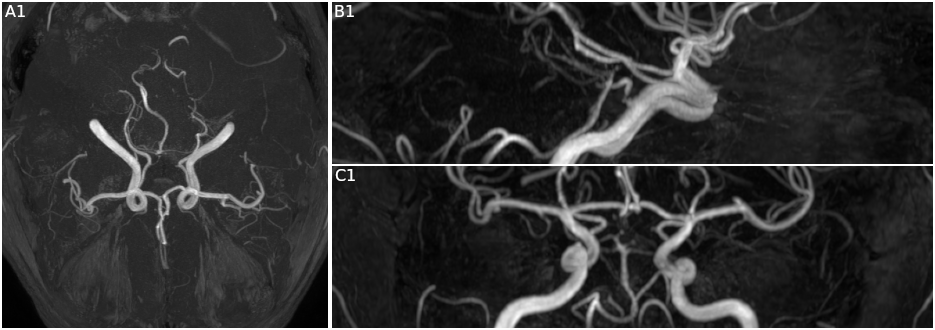
\includegraphics[width=\linewidth]{figures/mip_10021.png}
%		\phantomsubcaption
%		\label{fig:mip_10021.png}
	\end{subfigure}
	\begin{subfigure}{\linewidth}
		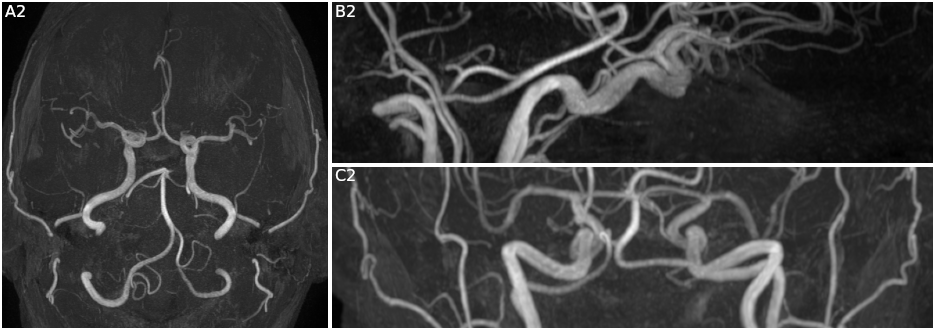
\includegraphics[width=\linewidth]{figures/mip_10028.png}
%		\phantomsubcaption
%		\label{fig:mip_10028.png}
	\end{subfigure}
	\caption[Maximum Intensity Projections of two positive cases.]{Images A1 and A2 show axial MIPs of two different cases that contain UIAs, and similarly B1, B2 and C1, C2 show sagittal and coronal views of MIPs respectively. The cases used are from the train dataset available via the ADAM challenge \cite{Timmins2020}.}
	\label{fig:mip}
\end{figure}

\begin{figure}[t]
	\centering
	\begin{subfigure}{\linewidth}
		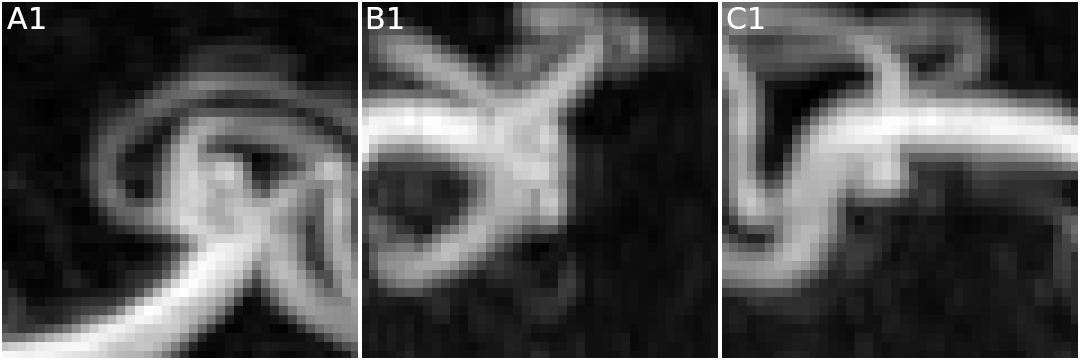
\includegraphics[width=\linewidth]{figures/mip_patch10021.png}
	\end{subfigure}
	\begin{subfigure}{\linewidth}
		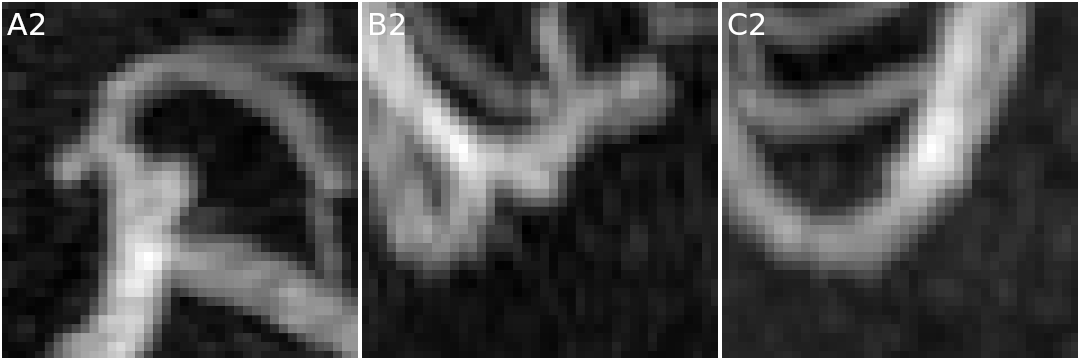
\includegraphics[width=\linewidth]{figures/mip_patch10028.png}
	\end{subfigure}
	\caption[Patches of Maximum Intensity Projections of two positive cases.]{Similarly to Figure \ref{fig:mip}, patches of axial, sagittal and coronal (A, B, and C) MIP images of two positives cases, are shown -- with the 3D patch from which the MIP is taken extracted with the aneurysm centered.}
	\label{fig:mip_patch}
\end{figure}


As discussed in chapter \ref{chapter3}, the size of aneurysms in a TOF-MRA is very small; the mean diameter of an aneurysm in our dataset being $4.11$ mm. With a re-sampled volume with voxel spacing $0.3 \times 0.3 \times 0.3$ mm\textsuperscript{3}, the mean shape of a volume encompassing an aneurysm would be $21.5 \times 21.5 \times 21.5$ -- assuming a spherical structure of the aneurysm. Axial, coronal and sagittal images (after preprocessing of the TOF-MRA volumes) would have shapes $512 \times 512$, $512 \times 140$, and $512 \times 140$ respectively. Due to this, an MIP taken of the whole three-dimensional TOF-MRA volume, would have little useful information regarding the aneurysm, such as an enlarged vessel. Therefore, as most other training procedures for other networks, Triplanar-Net is trained using patches of the whole volume. MIPs are then taken for the patch of cropped volume, further allowing the network to learn important features with respect to the aneurysm segmentation such as structure and shape. The projections the network learns from are thus as in Figure \ref{fig:mip_patch}, which are obtained from sampling a TOF-MRA volume. 

There are other projection methods, however using MIP for cerebral TOF-MRA is appropriate for this task due to the focus on vessels. \todo{is it ok to use MIP as projection method for brain volumes and why, what might be lost using 2D images, maybe contrast of TOF-MRA? etc}

\subsection{Network architecture}
The proposed Triplanar-Net is a CNN producing a binary segmentation the same size as the 3D patch used to create the MIPs. The model consists of an axial, coronal and sagittal 2D encoder path, a 2D to 3D reconstruction block, and a 3D decoder path, along with skip connections -- see the full architecture in Figure \ref{fig:trinet.pdf}. 

\img{trinet.pdf}{\linewidth}{Proposed network architecture for Triplanar-Net. Three input arms each take an MIP of either the axial, coronal or sagittal view extracted from a 3D patch. The inputs are encoded using 2D convolutions operations and max pooling before going through the 2D to 3D reconstruction block, and being decoded with 3D transpose convolutions followed by 3D convolutions. The convolution kernel size, padding size, and stride are represented as \{kernel.padding.stride\} in the image and the number of channels is shown within each block.}{Triplanar-Net architecture.}

\img{2d_to_3d.pdf}{0.5\linewidth}{Diagram of the 2D to 3D reconstruction block used in the Triplanar-Net architecture. Three inputs are given to the block -- representing the axial, sagittal and coronal MIPs. A 2D convolution with a kernel size of 3, padding 1 and stride 1 is applied to each input. The orthogonal views are then combined by taking the outer product, and a 3D convolution with kernel size of 3, padding 1 and stride 1 is applied to reconstructed 3D image.}{2D to 3D reconstruction block.}

In each encoder path a $1 \times 1$ convolution is applied to the respective input MIP, after which follow three layers containing $3 \times 3$ convolutions (with stride of 1 and padding 1) plus max-pooling with a stride of 2. 
In the the 2D to 3D reconstruction block, a convolution with kernel size $3 \times 3$ is applied to each of the feature maps of the axial, coronal and sagittal encoder paths. The 3D downsampled representation is constructed by calculating the outer product of the feature maps from the three orthogonal views, and applying a $3 \times 3 \times 3$ convolution. Figure \ref{fig:2d_to_3d.pdf} shows the 2D to 3D reconstruction block.
Lastly, to upsample the reconstructed 3D representation, the decoder path applies three layers of $4 \times 4 \times 4$ transpose convolutions (stride 2 and padding 1) followed by $3 \times 3 \times 3$ convolutions (stride 1 and padding 1). To take advantage of higher resolution features, skip connections are added that concatenate the output of each convolution operation in the encoder path to an equivalent decoder operation. As the decoder path incorporates three dimensional representations, the high-res features are also passed through their own 2D to 3D reconstruction block. The 3D binary voxelized segmentation of the aneurysm is obtained after applying a $1 \times 1 \times 1$ convolution. To introduce non-linearities to the model, each convolution operation (2D, 3D, and 3D transpose) with a kernel size greater than 1 is followed by an ELU activation function. Batch normalization is also applied after convolution operations (2D, and 3D) in the encoder and decoder paths.

Unlike the BtrflyNet architecture, Triplanar-Net constructs a 3D representation within the model (prior to the decoder path) and also does not contain a middle arm that concatenates the feature maps of the three encoder paths. Using a 3D decoder path allows the model to learn valuable 3D context when upsampling the naively reconstructed 3D feature maps, which would otherwise be lost if only 2D feature maps were involved. The parameters in the decoder path also allow to obtain a much more detailed binary segmentation, compared to that of a 2D decoder -- i.e. there would be a lot of aliasing when reconstructing a 3D output from three orthogonal MIP binary outputs for example, therefore it is more effective to create a reconstructed intermediate representation of the three projections within the network and obtain a 3D binary segmentation after decoding. 

As stated previously the axial, coronal and sagittal images used for training the network are obtained by finding the MIP in each view of a 3D patch cropped from the whole TOF-MRA volume. Multiple sampling schemes for extracting segments were tested; ultimately it was most successful to construct a training batch by extracting segments of size $32 \times 32 \times 32$ in which $90\%$ of the input samples correspond to background class and $10\%$ to foreground class (i.e. voxels containing an aneurysm). For cases in which there are no aneurysms in the TOF-MRA, all segments will only contain background class. This training strategy was employed as it reflects the most realistic distribution of foreground to background class within the data. The network is trained using dice loss which takes the form: 

\[L = 1 - \frac{2\sum_{i}^{N}p_{i}g_{i}}{\sum_{i}^{N}p_{i}^{2} + \sum_{i}^{N}g_{i}^{2}} \]

where $p_{i}$ and $g_{i}$ represent the voxel values of the predicted binary segmentation and the ground truth binary volume, summed over $N$ voxels \cite{milletari2016v}. The network is trained with 5-fold cross validation using the AdamW optimizer for 100 epochs per fold. L2 regularization of $1e-5$ is also used during training to reduce overfitting.

In comparison to the networks described in Chapter \ref{chapter4}, Triplanar-Net consists of a more shallow architecture, as well as both 2D and 3D convolutions. Generally, a shallower network can lead to poorer overall results be it for any task. However, by efficiently combining two dimensional and three dimensional data and convolutions, the network is able to be lightweight.  

Once trained, inference for a given input TOF-MRA volume proceeds as: segments of the volume are sampled on a grid, axial, coronal and sagittal MIPs are obtained for each segment and fed to the network. The output segmentation of the TOF-MRA volume is built by concatenating the network output of each segment.

%\todo{removed classifier/full pipeline part because think i can get it to work without}
%Training the network on only segments centered on the foreground (apart from negative cases) causes the network to produce segmentations with a high number of false-positives. To mitigate this as well as to allow Triplanar-Net to focus on accurate segmentation of aneurysms, it is proposed to add an initial classification step during inference on a TOF-MRA volume. The classifier evaluates whether a certain patch of the TOF-MRA volume contains a vessel with an aneurysm. If positively classified, the segment goes through to Triplanar-Net for aneurysm segmentation, and if negatively classified then no foreground pixels are segmented in the patch. The full framework for inference for any TOF-MRA volume can be seen in Figure \ref{full_pipeline.pdf}. The classifier network can also be seen in figure \todo{network for classifier}. The classifier network is trained on 3D segments of the same size as those used for training Triplanar-Net, using a uniform sampling scheme. We require that this classifier has a high sensitivity, and favors false-positives over false-negatives. Thus, it is trained using cross-entropy loss with a larger weight given to a positively classified volume. \info{elaborate/maybe write better}.
%
%\img{full_pipeline.pdf}{\linewidth}{\todo{caption}}{Full pipeline for inference.}
%
%Adding this classifier prior to Triplanar-Net is hypothesized to not heavily increase resource usage or heavily impede inference; most segments of the TOF-MRA volume will only go through one network (either the classifier or Triplanar-Net) since a very small number of segments (out of $N$ segments sampled from the TOF-MRA volume) contain an aneurysm. A segment is only processed by both the classifier and Triplanar-Net if an aneurysm is detected to be within it. The complete binary segmentation map for the TOF-MRA volume is then reconstructed by combining -- according to the coordinates of the sampled segment -- the $x$ binary segmentations from Triplanar-Net and $y$ binary segmentations that are known to not contain an aneurysm.
%
%An alternative to using this framework with a combined classifier and Triplanar-Net would be to use post-processing after obtaining the binary segmentation map of a segment and altogether not use the classifier at all. However, this was opted against as this \todo{Why not?}
%
%\todo{ablation study in appendix to show design choices, i.e. no skip blocks, no combination path, 2d decoders instead of 3d}





\chapter{Results}
\label{chapter6}
\todo{Aim for 6 to 7 pages}


\chapter{Discussion}
\label{chapter7}

In this study, two pre-existing networks were presented and used to assess the validity of our proposed network (Triplanar-Net), against a publicly available (train) dataset for cerebral UIA segmentation. Segmentation metrics are reported for both the train dataset and the non-publicly available dataset (test). The results shown for Triplanar-Net are lower than those reported for the SOTA -- the nnU-Net, however the network performs better than the well established DeepMedic network architecture. All three network architectures still show room for substantial improvement on the test dataset. Compared to the reported interobserver results by \citeauthor{Timmins2020}, the segmentation results are lower. It is also shown that in this study, it is possible to harvest 2D data and attempt to accurately reconstruct and learn 3D labels from it. 

The potential of neural networks to detect and segment UIAs in TOF-MRA's has been demonstrated previously, and the MICCAI2020 challenge presented by \citeauthor{Timmins2020} was an initiative that encouraged further exploration into this field. The steadily increasing workload of the radiology departments due to the growing necessity of radiological imaging must be managed; the introduction of more computer-aided diagnosis and detection tools in this regard can prove to show great improvement -- by possibly reducing diagnostic errors for example. \todo{Talk about segmentation explicitly}.

Based on the reported metrics, the results of the nnU-Net far surpass the results produced by DeepMedic and by Triplanar-Net on both the train dataset and the test dataset. With a Dice Score Coefficient of 0.81 on the train dataset the nnU-Net shows superior accuracy in terms of segmentation over DeepMedic and Triplanar-Net which have a DSC of 0.11 and 0.14 respectively. The Hausdorff distance is also the least for the nnU-Net architecture with 0.49 mm compared to large values of 59.70 mm for DeepMedic and 53.90 mm for Triplanar-Net (with values closer to 0 mm being the best). The high performance of the nnU-Net reported on the train dataset is also reflected in the test dataset with a DSC of 0.410 and a Hausdorff distance of 8.96, which both DeepMedic and Triplanar-Net could not surpass. The sensitivities of the three frameworks show some more similarities than the segmentation metrics, with nnU-Net outperforming DeepMedic and Triplanar-Net in the train dataset. However, DeepMedic shows to outperform both nnU-Net and Triplanar-Net with a sensitivity of 0.85 compared to 0.61 and 0.76 respectively. This could however be because of the large False Positive Count, i.e. DeepMedic has a fewer amount of false negatives due to the fact that it contains much more positive detections. In Figure \ref{fig:results} it is easily seen that the nnU-Net architecture also performs much more uniformly than DeepMedic and Triplanar-Net. Although there are some outliers in terms of DSC and VS for nnU-Net, both DeepMedic and Triplanar-Net show more variance in all cases, as well as more outliers so the segmentation accuracy is highly dependent for each individual case and could suggest that these networks were not able to generalize well on the dataset.

Triplanar-Net does outperform DeepMedic in all metrics across the board for both the train and test dataset -- with sensitivity being the only exception. The proposed network however cannot come near the results put forth by the SOTA. The average false positive count of Triplanar-Net particularly is much better than that of DeepMedic. \todo{why? so what? also related: why deepmedic performs so much worse on this dataset}

Taking a look at the results of the further evaluations: considering inference time of each network, nnU-Net is very resource intensive with almost 150 times more parameters than both DeepMedic and Triplanar-Net. Using a larger network -- one with more parameters -- is most likely one of the reasons the nnU-Net outperforms both the other two networks. nnU-Net and DeepMedic both use only 3D convolutions, and thus the inference time per case (not including pre- and postprocessing) is much larger than that of Triplanar-Net which combines the use of both 2D and 3D convolution operations. It is surprising that DeepMedic contains a slightly smaller amount of parameters than Triplanar-Net but takes almost the same amount of inference time as nnU-Net; this could be accounted by the parameters introduced in Triplanar-Net by adding the skip connections which are not present in DeepMedic. Even though the time to infer could be considered a valuable metric if an automated system is employed in a real-time clinical setting, if the segmentation accuracy cannot be on par with the SOTA then this cannot be deemed an important factor, and the same can be said for the number of parameters.

Evaluating segmentation performance of the networks on only true positive detections also made an impact: both the DSC and MHD are seen to improve for the DeepMedic architecture and for the Triplanar-Net architecture. The nnU-Net framework nonetheless still outperforms the other two architectures. It is interesting to note that DeepMedic outperforms Triplanar-Net in all metrics when only considering true UIAs, showing that the accuracy of the segmentation if ignoring any false positives is actually slightly better than Triplanar-Net. When taking a further look into the performance on negative scans, it can be seen that DeepMedic has the highest number of False positives for both negative and positive cases, with the false positive count for negative scans being drastically greater than that for positive scans. The nnU-Net framework detects 0 false positives throughout all scans in the train dataset which is an impressive feat; although Triplanar-Net does not have a large variance between false positives on positive and negative scans, the number is still large in and of itself. \todo{Mention false positive count with respective to detections by radiologists}

Taking a look at Figure \ref{fig:qual_results} it can be seen that all three network architectures show better DSCs for cases with larger aneurysm sizes. The nnU-Net framework also seems to struggle for very small aneurysms (even though the mean DSC value for small aneurysms is around 0.80). Although both DeepMedic and Triplanar-Net do show better performance for larger aneurysms (with a median of around 0.20 and 0.38 respectively) the box plots show a large inter-quartile range, i.e. the results are not very uniform in those instances.

The performance of nnU-Net shows to drop drastically between the train dataset and the test dataset, suggesting that although the framework shows exceptional performance on the train dataset it may not be able to generalize well to the test dataset. Although nnU-Net performed better with respect to the DSC and MHD, Triplanar-Net showed a better Volumetric Similarity for test dataset. The Triplanar-Net and DeepMedic architectures also reported a much smaller difference in segmentation metrics on the train and test dataset. As stated by \citeauthor{Timmins2020} the characteristics such as the distribution of aneurysms of the train and test dataset are similar, so the train dataset is ensured to be representative of the test dataset. Therefore the reason for the poorer performance could lie in factors such as the train/validation split during training, aneurysm sizes. However it is also difficult to account for changes in aneurysm shapes or differences in parent vessels. In a clinical setting the uniformity of images and conditions cannot be replied upon and so ideally methods should be able to detect and segment UIAs on unseen examples too.

The axial slices of the three cases in Figure \ref{fig:qual_results} show once again the superior performance of the nnU-Net architecture over DeepMedic and Triplanar-Net: the shape of the aneurysm is captured more accurately, and there are no false positive detections. Triplanar-Net and DeepMedic both do seem to detect an aneurysm in similar locations to nnU-Net but the segmentation itself is lacking.

With these results before us it can be said that Triplanar-Net does not perform as expected, and that attempting to segment aneurysms in 3D TOF-MRA images using 2D MIP views was not successful. Although Triplanar-Net performs almost on par with DeepMedic -- which is a 3D network -- it can be said that the loss of 3D context while using Triplanar-Net was its downfall. Although the use of 2D MIPs in the case of spine CT images seems to show good results for the Btrfly-Net, the task of aneurysm segmentation is much more imbalanced. The task of aneurysm segmentation in TOF-MRA images is itself a hard one, and attempting to reduce the number of parameters and improve on inference time for use in a clinical setting was not possible as the network could not generalize well. Some small changes such as making the architecture deeper or increasing the number of feature maps in each layer are possible future areas of work, however the area most in need of improvement and/or further testing could be the 2D to 3D reconstruction block. Different ensembles could also be tested for further justification or proof of concept in this regard. Much like many other deep learning methods, an increase in the number of cases used to train the network could also be a valuable area of future exploration. 

\todo{Discuss why DeepMedic performed much worse on this dataset than in their own study}
\todo{Possible reasons why my network sucks ass}
\todo{Future work in this regard, is it still viable to use 2D for 3D data}






\chapter{Conclusion}
\label{chapter8}
This study could not demonstrate that the proposed Triplanar-Net could perform on par with the SOTA to segment UIAs in TOF-MRA images. A dataset comprising of both positive, and negative scans, acquisitions of varying field strengths, varying image quality, and varying voxel sizes was used, which was made available as part of the MICCAI2020 ADAM challenge run by \citeauthor{Timmins2020}. The dataset is a difficult one to perform accurate segmentations on, as made clear by the fact that DeepMedic -- another network evaluated on the dataset -- performed poorly as compared to the study carried out by \citeauthor{Sichermann2019} with their own in-house dataset. 

The concept of using 2D MIPs taken of patches of 3D volumes is an approach that has not been deeply explored in this setting, especially if a 3D segmentation is the required output. Reconstructing a 3D volume from the projections is a challenge, however the proposed network was able to introduce some learned parameters to the reconstruction to attempt to improve on the naive method of reconstructing using the outer product. 

In the future, further development of methods for segmentation of UIAs will be required before being able to accurately segment and quantify UIAs automatically in TOF-MRA images, at least to the same level as that possible of a radiologist.




% #################
% ### APPENDIX  ###
% #################

\chapter*{Acknowledgments}
%\addcontentsline{toc}{chapter}{Acknowledgments}
\thispagestyle{empty}

I would like to thank my advisor Supro for his technical support and his suggestions and ideas. The author of the ADAM challenge, Kimberley, was very responsive and helpful when first using the dataset and evaluating it on the test dataset. I would also like to thank Alessa, Luis and Saif for reading and going over my thesis and being as judgmental as they were without being cynical -- especially Alessa and Luis who also cooked food when I couldn't. I would also like to thank everyone in the IBBM research group for putting up with me using a lot of GPU resources for a while. Finally, I would like to thank my parents for always being there even when I went MIA for a few weeks at a time.

\cleardoublepage{}


%\part*{Appendix}
%
%\pagenumbering{Roman} % römische Ziffern für die Anhänge
%
%\begin{appendix}
%	\chapter{Appendix: Ablation study for network architecture design}
\label{appendix1}

Before arriving to the network architecture shown in Chapter \ref{chapter5} for Triplanar-Net, other network architectures were also designed with the same concept of attempting to employ the use of 2D MIPs to segment aneurysms in 3D TOF-MRA images. In particular, the BtrflyNet architecture, the BtrflyNet with an added third input arm -- Figure \ref{fig:triflynet.pdf}, and the BtrflyNet with a 3D decoder substituting the 2D decoder -- Figure \ref{fig:3dtriwingednet.pdf} were the networks tested. Small variations of these networks were also tested, such as removing the skip connection or varying the channels in each layer. All these architectures proved to not be able to even overfit well enough on data used to train the architecture, and thus the final iteration of Triplanar-Net was decided upon. The DSC of each network evaluated on full volumes of the cases used to train the network are shown in Table \ref{table:iterations}. Only the DSC is reported so as to only to show one necessary metric to evaluate the segmentation performance.

\img{triflynet.pdf}{\linewidth}{Design iteration 1. Proposed architecture for variation of BtrflyNet with an additional third input arm, taking inputs as axial, coronal and sagittal MIPs and obtaining axial, coronal and sagittal MIP labels.}{Design iteration 1.}

\img{3dtriwingednet.pdf}{\linewidth}{Design iteration 2. Proposed architecture for variation of design iteration 1 using a 2D to 3D reconstruction block and a 3D decoder.}{Design iteration 2.}

\begin{table}[htp]
	\centering
	
	\begin{tabular}{l | r}
		& DSC \\
		\hline
		Design iteration 1 & 0.14 \\
		Design iteration 1 (no skip) & 0.09 \\
		Design iteration 2 & 0.23 \\
		Design iteration 2 (with skip) & 0.37 \\
		Triplanar-Net & \textbf{0.62}
	\end{tabular}

	\caption[Evaluation on training data for architecture designs before Triplanar-Net.]{DSCs reported for full volumes of training data for design iterations and variations.}
	\label{table:iterations}
\end{table}

The issue with design iteration 1 was presumed to be that the complete loss of 3D context within this architecture manifests in a poor performing network; having to reconstruct the 3D binary output segmentation after obtaining the 2D MIP labels of each view could be changed to allow combining of the three labels in a less naive method. Therefore, it was opted to change to design iteration 2, in which a 3D decoder is used after reconstructing the 3D labels within the network using the 2D to 3D reconstruction block as mentioned in Chapter \ref{chapter5}. It was also interesting to see the addition and removal of skip connections in design iteration 2. Finally, to arrive at the chosen design for Triplanar-Net, the middle arm of design iteration 2 was removed as concatenating the intermediate features of the three input arms was hypothesized to not be a useful use of the processed features.

A further experiment was also carried out to use a 2-staged pipeline to segment aneurysms. The first stage being localizing the aneurysm, and the second stage involving the actual segmentation. The pipeline can be seen in Figure \ref{fig:full_pipeline.pdf}. The hope with using this 2-stage pipeline was to reduce false positives. In the end, although various architectures were attempted for the first stage, the specificity and sensitivity were too low to warrant using a 2-staged approach for the task. If a classifier network is unable to detect accurately enough whether a certain patch contains an aneurysm, than the chance of false negatives for the full pipeline would be drastically increased. This pipeline was experimented with various classifier networks and segmentation networks (with the iterations discussed), and the maximum sensitivity and specificity achieved (for the first stage) was 0.84 and 0.77 respectively.

\img{full_pipeline.pdf}{\linewidth}{Proposed 2-staged pipeline, incorporating classification of a specific input patch before performing segmentation. The hope is to reduce false positives, while not drastically increasing workload and amount of required resources.}{Proposed 2-staged pipeline for inference.}




		
%\end{appendix}

% Reset paragraph whitespace
\bigLineSpacing{OFF}

 \glsaddall{} % add all defined terms to glossary, even if not referenced in text
 \printglossaries{}
 
 \microtypesetup{protrusion=false}
 \listoffigures{}
 \listoftables{}
 \microtypesetup{protrusion=true}
 \printbibliography{}

\end{document}
